\subsection{Continuous-Discrete Extended Kalman Filter}
The Continuous-Discrete Extended Kalman Filter (\textit{CDEKF}) consists of a time update (\cref{eq:CDEFK_time} and a measurement update (\cref{eq:CDEFK_meas}). The advantage of using a \textit{CDEKF} is the fact that the filter uses the non-linear model to estimate the states, where the clasical Kalman filter uses the linearized model.\\
Time update:
\begin{equation}
\label{eq:CDEFK_time}
    \begin{gathered}
        \hat{y}_{k|k-1}=g(\hat{x}_{k|k-1},\theta) \qquad C_k=\frac{\partial g}{\partial x}(\hat{x}_{k|k-1},\theta)\\
        e_l=y_k-\hat{y}_{l|k-1}\\
        R_{e,k}=C_kP_{k|k-1}C_k^T+R_k\\
        \hat{x}_{k|k}=\hat{x}_{k|k-1}+K_ke_k\\
        K_k=P_{k|k-1}C_k^TR_{e,k}^{-1}\\
        P_{k|k}=P_{k|k-1]}-K_kR_{e,k}K_k^T
    \end{gathered}
\end{equation}
Measurement update:
\begin{equation}
    \begin{gathered}
        \frac{dx(t)}{dt}=f\Big(\hat{x}_k(t),u_k,d_k,\theta\Big)\qquad\hat{x}_k(t_k)=\hat{x}_{k|k}\\
        \frac{dP_k(t)}{dt}=A_k(t)P_k(t)+P_k(t)A_k(t)^T\sigma_k(t)\sigma_k(t)^T\qquad P_k(t_k)=P_{k|k}\\
        A_k(t)=\frac{\partial f}{\partial x}\Big(\hat{x}_k(t),u_k,d_k,\theta\Big)\\
        \sigma_k(t)=\sigma\Big(\hat{x}_k(t),u_k,d_k,\theta\Big)
    \end{gathered}
\label{eq:CDEFK_meas}
\end{equation}
The implementation of the \textit{CDEKF} is implemented as seen in \cref{app:CDEKF}. The simulation of the system can be seen in the below figure. Notice that it is the states (hence the units is in gram), since these clearly visualize the non-linearity of the system where outputs in cm is purely a scaling. The system is initialized from steady state and a step change occurs in the input at time 10 and 20 minutes. 
\begin{figure}[H]
    \centering
    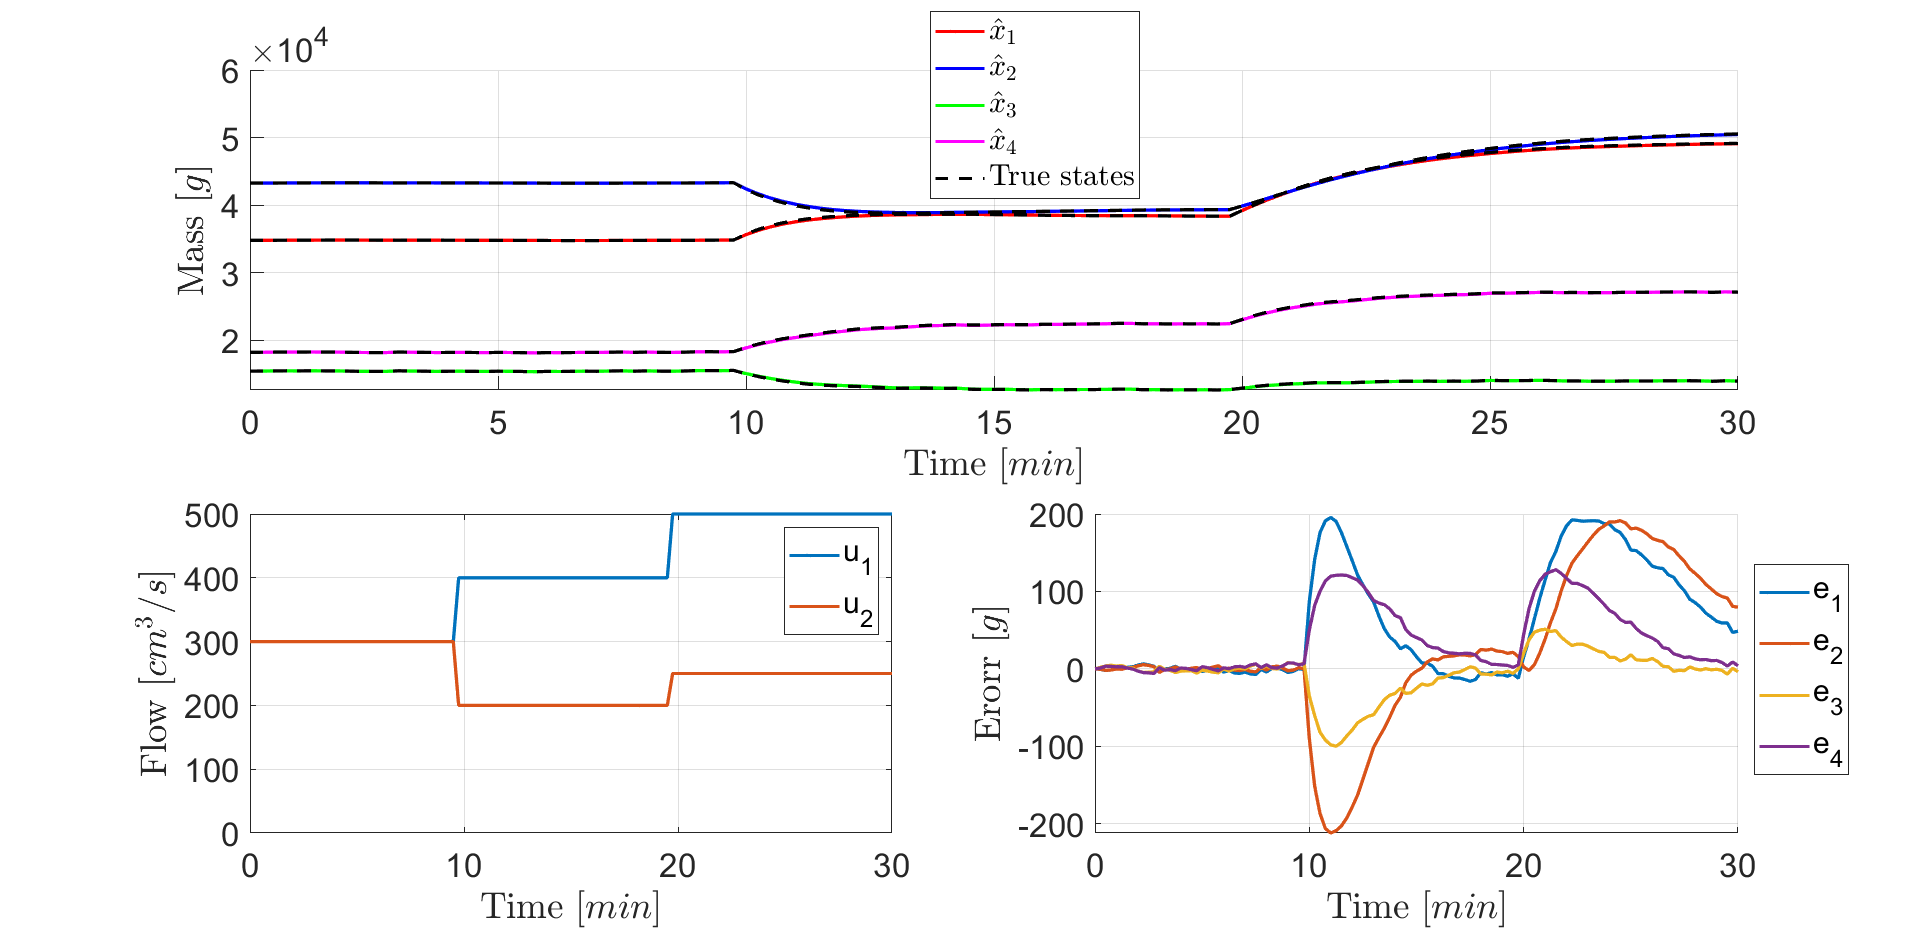
\includegraphics[width=1\textwidth]{Figures/Pr11.2_CDEKF.png}
    \caption{CDEKF implementation}
    %\label{fig:Kalman_stoc_state_step}
\end{figure}
It can be seen that the error between the true state and the estimated states are relatively small, even though the steps forces the system to move far from the steady state point.